\section{Choisir la source du fichier/assigner les colonnes}
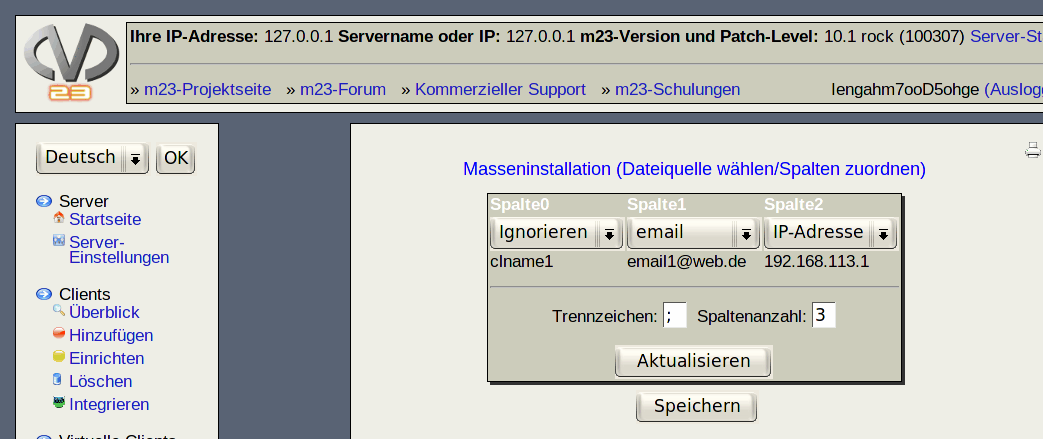
\includegraphics[scale=0.33]{/mdk/doc/manual/screenshots/fr/mi_step2.png} \\
Ce dialogue est partag\'e en deux pas:\\
\begin{itemize}
\item Choisir le fichier et le t\'el\'echarger\\
\item Assigner les propri\'et\'es du poste client aux cases du fichier\\
\end{itemize}
\subsection{Choisir le fichier et le t\'el\'echarger}
Choisissez un fichier par le dialogue et puis, cliquez sur \textit{$\ll$T�l�charger vers le serveur$\gg$}.\\
Le fichier doit \^etre construit sp\'ecialement, pour que m23 puisse identifier les valeurs. Dans chaque ligne, les valeurs des propri\'et\'es d'un seul poste client sont sp\'ecifi\'ees. Chaque propri\'et\'e est s\'epar\'e des autres par un signe de s\'eparation (ici: $\ll$;$\gg$): \\
\begin{verbatim}
propri\'et\'e1;propri\'et\'e2;propri\'et\'e3;...
\end{verbatim}
Au lieu d'un point-virgule, vous pouvez utiliser n'importe quelle combinaison d'un maximum de 4 lettres/chiffres. L'ordre des propri\'et\'es doit \^etre le m\^eme dans chaque ligne.\\
\subsection{Notez}
\`A part de la condition fondamentale que les valeurs entr\'ees dans le fichier doivent \^etre harmonis\'ees avec les propri\'et\'es, il y a ces conditions additionnelles pour les propri\'et\'es suivantes:\\
\begin{itemize}
\item \textbf{Enregistrer les donn�es d'ouverture de session local sur le poste client.}: Avec la valeur $\ll$yes$\gg$, vous activez cette option, toutes autre valeur la d\'esactive.\\
\item \textbf{LDAP}: 3 valeurs diff\'erentes sont admissibles:\\
\begin{itemize}
\item $\ll$none$\gg$: Ne pas utiliser le LDAP\\
\item $\ll$read$\gg$: Lire les donn�es d'ouverture de session du serveur LDAP s�lectionn�.\\
\item $\ll$write$\gg$: Enregistrer les donn�es d'ouverture de session sur le serveur LDAP.\\
\end{itemize}
\end{itemize}
\subsection{Assigner les propri\'et\'es du poste client aux cases du fichier}
Apr\`es que vous avez t\'el\'echarg\'e un fichier, vous pouvez assigner les propri\'et\'es de vos postes client aux cases du fichier.\\
\subsection{Proc\'edez comme c'est d\'ecrit au suivant:}
\begin{enumerate}
\item Entrez votre signe de s\'eparation dans la case et adaptez le nombre de colonnes si c'est n\'ecessaire.\\
\item Cliquez sur \textit{$\ll$Actualiser$\gg$}.\\
\item Assignez les propri\'et\'es de vos postes client dans les listes aux cases du fichier de la banque de donn\'ees.\\
\item Enregistrez votre s\'election par un clic sur \textit{$\ll$Enregistrer$\gg$}.\\
\end{enumerate}
